\documentclass[Royal,times,sageh]{sagej}

\usepackage{moreverb,url,natbib, multirow, tabularx}
\usepackage[colorlinks,bookmarksopen,bookmarksnumbered,citecolor=red,urlcolor=red]{hyperref}





\begin{document}

\title{Missing the Point\(\colon\) Non-Convergence in Iterative Imputation
Procedures}

\runninghead{Oberman}

\author{H. I. Oberman\affilnum{1}}

\affiliation{\affilnum{1}{Department of Methodology and Statistics, Utrecht University, Utrecht,
The Netherlands}}

\corrauth{Hanne Oberman, Sjoerd Groenman building, Utrecht Science Park, Utrecht,
The Netherlands.}

\email{\href{mailto:h.i.oberman@uu.nl}{\nolinkurl{h.i.oberman@uu.nl}}}

\begin{abstract}
(\textbf{Rewrite:}) Multiple imputation by chained equations (MICE) is a
widely used tool to accommodate missing data. While empirical evidence
supports the validity of inferences obtained using mice, there is no
consensus on the convergence properties of the method. This paper
provides insight into non-convergence of mice algorithms.
\end{abstract}

\keywords{MICE; convergence}

\maketitle

\textbf{Note for peer review: things written in bold are reminders for
myself or things that I am unsure off still. Also, I just decided to
change things majorly in my results section. So right now, the figures
do not correspond to the text. Please only skim that section, because I
am definitely going to rewrite it. Thanks already! - Hanne}

\hypertarget{introduction}{%
\section{Introduction}\label{introduction}}

Missing data problems are ubiquitous and pervasive in the social and
behavioral sciences. If a dataset contains just one missing value for a
variable of interest, statistical inferences are undefined and will not
produce any result. Incomplete observations are therefore ignored by
default in many statistical packages (i.e., list-wise deletion is
employed). Unfortunately, this \emph{ad hoc} solution may yield wildly
invalid results \citep{buur18}. An alternative is to `impute' (i.e.,
fill in) every missing value in an incomplete dataset. With imputation
techniques, one or several completed datasets are created, on which
statistical inferences can be performed. The case with several completed
datasets is known as `multiple imputation' \citep[MI;][]{rubin76}, and
requires an additional step to pool the results across imputations
\textbf{see figure 1??}.

\textbf{Move this after notation??} Figure 1 provides an overview of the
steps involved with MI---from incomplete data, to \(M\) completed
datasets, to \(M\) estimated quantities of interest (\(\hat{Q}\)s), to a
single pooled estimate \(\bar{Q}\). Missing data in \(y\) is `imputed'
(i.e., filled in) \(M\) times. The imputed data (\(y_{imp}\)) is
combined with the observed data (\(y_{obs}\)) to create \(M\) completed
datasets. On each completed dataset, the analysis of scientific interest
(the `substantive model', or `complete data model') is performed. The
quantity of scientific interest (e.g., a regression coefficient) is
denoted with \(Q\). Since \(Q\) is estimated on each completed dataset,
\(M\) separate \(\hat{Q}\)-values are obtained. These \(M\) values are
combined into a single pooled estimate \(\bar{Q}\). \textbf{ALSO: make
clear that iteration happens within the first step.}

\begin{figure}

{\centering 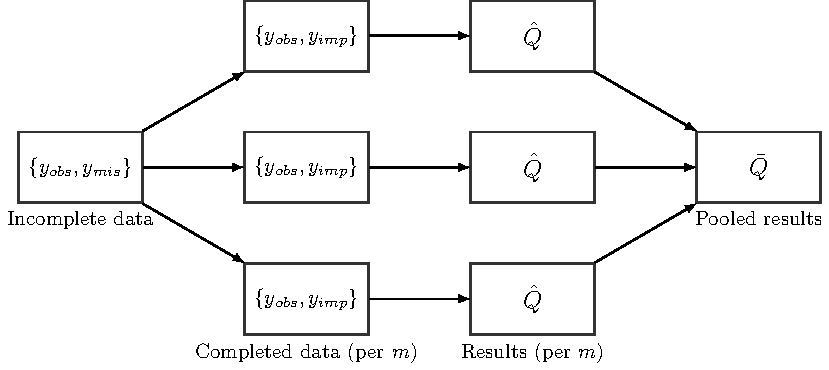
\includegraphics[width=\linewidth]{./images/diagram} 

}

\caption{Scheme of the main steps in multiple imputation.}\label{fig:unnamed-chunk-1}
\end{figure}

By applying Rubin's rules, the pooled result will reflect the
uncertainty in the data due to missingness. Under many circumstances,
this yields an unbiased and confidence valid estimate of the inference
on the true--but missing--data \citep{buur18}. A popular method to
obtain imputations is to use the `Multiple Imputation by Chained
Equations' algorithm, shorthand `MICE'\citep{mice}. MICE is an iterative
algorithmic procedure to draw imputations from the posterior predictive
distribution of the missing values. This introduces a potential threat
to the validity of the imputations: what if the algorithm has not
converged? Are the implications then to be trusted? And can we rely on
the inference obtained on the completed data? These are all open
questions, because the convergence properties of iterative imputation
algorithms have not been systematically studied \citep{buur18}.
Moreover, there is no scientific consensus on the convergence properties
of MI algorithms \citep{taka17}. Some default MICE techniques (e.g.,
`predictive mean modeling') might not yield converged states at all
\citep{murr18}. Therefore, algorithmic convergence should be monitored
carefully.

The recommended practice to monitor convergence is to visually inspect
imputations for signs of non-convergence. This practice is insufficient
on two counts: 1) it may be challenging to the untrained eye, and 2)
only severely pathological cases of non-convergence may be diagnosed
\citep[\(\S\) 6.5.2]{buur18}. Therefore, a quantitative, diagnostic
evaluation of convergence would be preferred.

Iterative imputation algorithms such as MICE are Markov chain Monte
Carlo (MCMC) methods, which means that convergence is not from a scalar
to a point but from one distribution to another. The values generated by
the algorithm (e.g., imputed values) will vary even after convergence.
Therefore, the aim of convergence diagnostics for MCMC methods should
not be to establish the point at which convergence is reached, but to
monitor signs of non-convergence. Several convergence diagnostics for
MCMC methods exist, but it is not known whether these are appropriate
for MICE.

Main question: How can non-convergence be diagnosed? Sub-questions: Are
common MCMC non-convergence diagnostics appropriate for MICE? And if so,
which threshold should be used to diagnose non-convergence? How many
iterations are sufficient/needed to be able to diagnose non-convergence?
Are the default number of iterations sufficient (i.e., 5 in mice, 10 in
SPSS and Stata, 30 in mi)? \textbf{(These are part of the methods, not
RQ per se: What are the effects of continued iterations on estimates,
predictions and inferences? And finally, do the answers differ with
varying missingness proportions? That is, we vary the nr of iterations
and the missingness proportion because we assume that the algorithm has
not reached convergence at \(t=1\), and performs worse with moderate to
high missingness (not so much with little or a LOT of missingness).)}

For reasons of brevity, we only focus on the MI algorithm implemented in
the world-leading MI software: the \texttt{R} \citep{R} package
\texttt{mice} \citep{mice}. The convergence properties of this MI
algorithm are investigated through model-based simulation. The results
of this simulation study are guidelines for assessing convergence of MI
algorithms, which will aid applied researchers in drawing valid
inference from incomplete datasets.

\hypertarget{notation}{%
\subsection{Notation}\label{notation}}

Let \(y\) denote an \(n \times p\) matrix containing the data values on
\(p\) variables for all \(n\) units in a sample. The data value of unit
\(i\) (\(i = 1, \dots, n\)) on variable \(j\) (\(j = 1, \dots, p\)) may
be either observed or missing. The collection of observed data values in
\(y\) is denoted by \(y_{obs}\); the missing part of \(y\) is referred
to as \(y_{mis}\). For each datapoint in \(y_{mis}\), we sample
\(M \times T\) times plausible values, where \(M\) is the number of
imputations (\(m = 1, 2, \dots, M\)) and \(T\) is the number of
iterations (\(t = 1, 2, \dots, T\)). The collection of samples between
the initial value (at \(t=1\)) and the final imputed value (at \(t=T\))
will be referred to as an `imputation chain'. \textbf{Add: missingness
percentage = proportion of cases with one or more missing values, Q is
quantity of scientific interest: ``A scientific estimand \(Q\) is a
quantity of scientific interest that we can calculate if we would
observe the entire population'' \citep[par 2.3.1]{buur18}. }

\hypertarget{convergence-diagnostics}{%
\section{Convergence diagnostics}\label{convergence-diagnostics}}

The two challenges for convergence of iterative algorithms are mixing
and stationarity \citep{gelm13}, see Figure XYZ. Without mixing,
imputation chains do not intermingle nicely. Without stationarity, there
is trending within imputation chains. While the current practice is to
inspect traceplots for signs of non-mixing and non-stationarity,
diagnostic evaluation of these two challenges would be preferred.
Non-stationarity within chains may be diagnosed with e.g.,
autocorrelation \citep[\(AC\);][]{scha97, gelm13}, numeric standard
error \citep[`MC error';][]{gewe92}, or Raftery and Lewis's
\citeyearpar{raft91} procedure to determine the effect of trending on
the precision of estimates. A widely used diagnostic to monitor mixing
between chains is the potential scale reduction factor \(\widehat{R}\)
\citep[`Gelman-Rubin statistic';][]{gelm92}. With a recently proposed
adaptation, \(\widehat{R}\) might also serve to diagnose
non-stationarity, but this has not yet been thoroughly investigated
\citep{veht19}. Therefore, mixing and stationarity will be evaluated
separately in this study. As recommended \citep[e.g.,][p.~898]{cowl96},
\(AC\) and \(\widehat{R}\) will be used.

\begin{figure}

{\centering 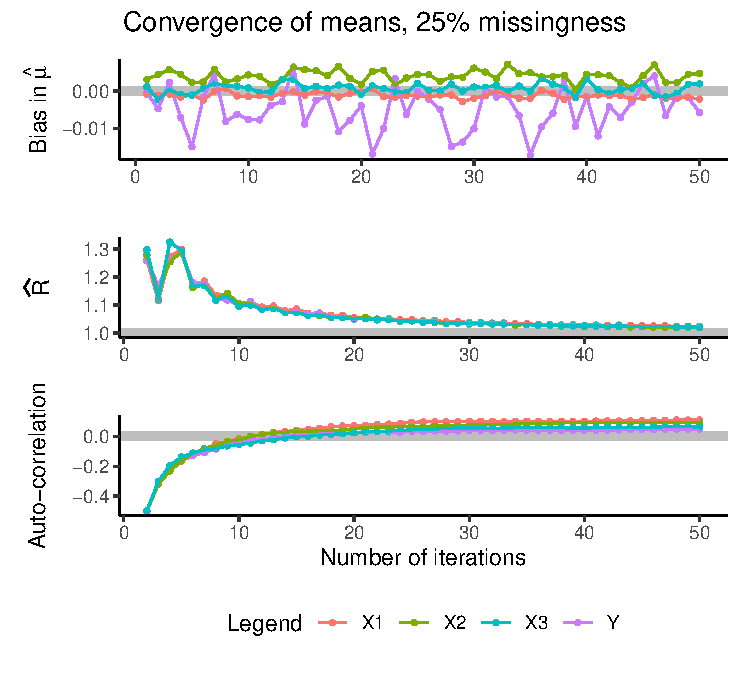
\includegraphics[width=.49\linewidth]{manuscript_files/figure-latex/unnamed-chunk-2-1} 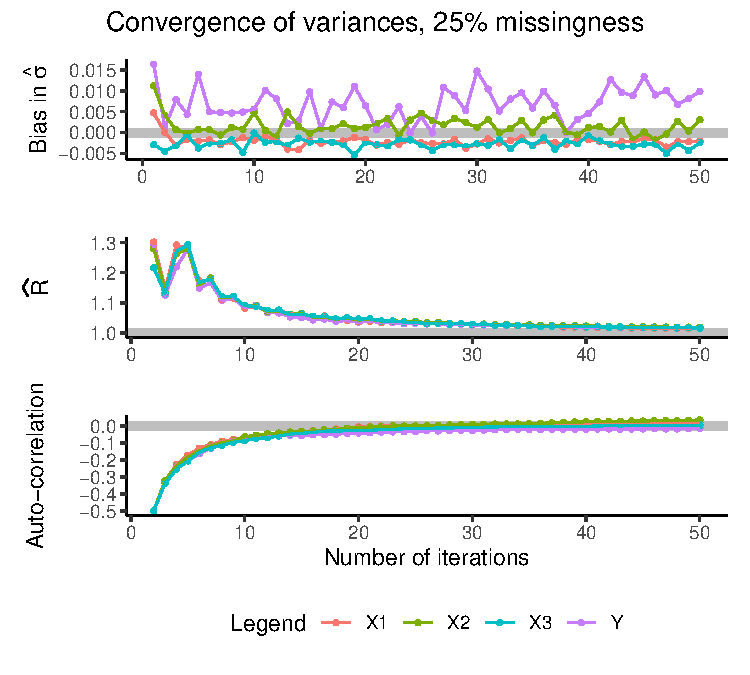
\includegraphics[width=.49\linewidth]{manuscript_files/figure-latex/unnamed-chunk-2-2} 

}

\caption{Pathological non-convergence versus typical convergence.}\label{fig:unnamed-chunk-2}
\end{figure}

\hypertarget{potential-scale-reduction-factor}{%
\subsection{Potential scale reduction
factor}\label{potential-scale-reduction-factor}}

To define \(\widehat{R}\), we follow notation by \citep[p.~5]{veht19}.
Let \(M\) be the total number of chains, \(T\) the number of iterations
per chain, and \(\theta\) the scalar summary of interest (e.g., chain
mean or chain variance). For each chain (\(m = 1, 2, \dots, M\)), we
estimate the variance of \(\theta\), and average these to obtain
within-chain variance \(W\).

\begin{align*}
W&=\frac{1}{M} \sum_{m=1}^{M} s_{j}^{2},  \text { where } s_{m}^{2}=\frac{1}{T-1} \sum_{t=1}^{T}\left(\theta^{(t m)}-\bar{\theta}^{(\cdot m)}\right)^{2}. 
\end{align*}

We then estimate between-chain variance \(B\) as the variance of the
collection of average \(\theta\) per chain.

\begin{align*}
B&=\frac{T}{M-1} \sum_{m=1}^{M}\left(\bar{\theta}^{(\cdot m)}-\bar{\theta}^{(\cdot \cdot)}\right)^{2}, \text { where } \bar{\theta}^{(\cdot m)}=\frac{1}{T} \sum_{t=1}^{T} \theta^{(t m)} \text{, } \bar{\theta}^{(\cdot \cdot)}=\frac{1}{M} \sum_{m=1}^{M} \bar{\theta}^{(\cdot m)}. 
\end{align*}

From the between- and within-chain variances we compute a weighted
average, \(\widehat{\operatorname{var}}^{+}\), which over-estimates the
total variance of \(\theta\) \textbf{remove or explain why}.
\(\widehat{R}\) is then obtained as a ratio between the over-estimated
total variance and the within-chain variance:

\begin{equation*}
\widehat{R}=\sqrt{\frac{\widehat{\operatorname{var}}^{+}(\theta | y)}{W}},
\text{ where } \widehat{\operatorname{var}}^{+}(\theta | y)=\frac{N-1}{N} W+\frac{1}{N} B.
\end{equation*}

We can interpret \(\widehat{R}\) as potential scale reduction factor
since it indicates by how much the variance of \(\theta\) could be
shrunken down if an infinite number of iterations per chain would be run
\citep{gelm92}. This interpretation assumes that chains are
`over-dispersed' at \(t=1\), and reach convergence as \(T \to \infty\).
Over-dispersion implies that the initial values of the chains are `far
away' from the target distribution and each other. When all chains
sample independent of their initial values, the mixing component of
convergence is satisfied, and \(\widehat{R}\)-values will be close to
one. High \(\widehat{R}\)-values thus indicate non-convergence. The
conventionally acceptable threshold for convergence was
\(\widehat{R} < 1.2\) \citep{gelm92}. More recently, \citet{veht19}
proposed a more stringent threshold of \(\widehat{R} < 1.01\).

\hypertarget{autocorrelation}{%
\subsection{Autocorrelation}\label{autocorrelation}}

Following the same notation, we define autocorrelation as the
correlation between two subsequent \(\theta\)-values within the same
chain \citep[p.~147]{lync07}. In this study we only consider \(AC\) at
lag 1, i.e., the correlation between the \(t^{th}\) and \(t+1^{th}\)
iteration of the same chain.

\begin{equation*}
AC = \left( \frac{T}{T-1} \right) \frac{\sum_{t=1}^{T-1}(\theta_t - \bar{\theta}^{(\cdot m)})(\theta_{t+1} - \bar{\theta}^{(\cdot m)})}{\sum_{t=1}^{T}(\theta_t - \bar{\theta}^{(\cdot m)})^2}.
\end{equation*}

We can interpret \(AC\)-values as a measure of stationarity. If
\(AC\)-values are close to zero, there is no dependence between
subsequent samples within imputation chains.

Positive \(AC\)-values indicate recurrence. If \(\theta\)-values of
subsequent iterations are similar, trending may occur. Negative
\(AC\)-values show no threat to the stationarity component of
convergence. On the contrary even---negative \(AC\)-values indicate that
\(\theta\)-values of subsequent iterations diverge from one-another,
which may increase the variance of \(\theta\) and speed up convergence.
As convergence diagnostic, the interest is therefore in positive
\(AC\)-values. Moreover, the magnitude of \(AC\)-values may be evaluated
statistically, but that is outside of this note's scope.

Negative \(AC\)-values indicate divergence within imputation chains.
\textbf{Subsequent sampled values within each imputation chain are less
alike.}

In short, convergence is reached when there is no dependency between
subsequent iterations of imputation chains (\(AC = 0\)), and chains
intermingle such that the only difference between the chains is caused
by the randomness induced by the algorithm (\(\widehat{R} = 1\)).

\hypertarget{simulation-hypothesis}{%
\subsection{Simulation Hypothesis}\label{simulation-hypothesis}}

This study evaluates whether \(\widehat{R}\) and \(AC\) could diagnose
convergence of multiple imputation algorithms. We assess the performance
of the two convergence diagnostics against the recommended evaluation
criteria for MI methods \citep[i.e., average bias, average confidence
interval width, and empirical coverage rate across simulations;][\(\S\)
2.5.2]{buur18}. That is, there is no baseline measure available to
evaluate performance against.

Based on an empirical finding \citep{lace07}, we hypothesize that
\(\widehat{R}\) will over-estimate non-convergence of MI algorithms
\textbf{explain why?}. The threshold of \(\widehat{R} < 1.01\) will then
be too stringent for diagnosing convergence. This over-estimation may,
however, be diminished because \(\widehat{R}\) can falsely diagnose
convergence if initial values of the algorithm are not appropriately
over-dispersed \citep[p.~437]{broo98}. In \texttt{mice}, initial values
are chosen randomly from the observed data. Therefore, we cannot be
certain that the initial values are over-dispersed. We expect this to
have little effect on the hypothesized performance of \(\widehat{R}\)
\textbf{explain that the randomness induced by the MICE algorithm would
take care of this??}. \textbf{(Add actual hypothesis: we thought that
mice would converge sooner than \(\widehat{R}\) would indicate that it
did)} No hypothesis was formulated about the performance of \(AC\) as
convergence diagnostic. \textbf{Added later: High \(AC\)-values are
implausible in MI procedures. That is, the randomness induced by the MI
algorithm effectively mitigates the risk of dependency within chains.}

\hypertarget{simulation-study}{%
\section{Simulation study}\label{simulation-study}}

Research question when and how to diagnose non convergence?

QUESTION: How?

The two challenges of convergence are stationarity and mixing point.
Mixing and stationarity can be evaluated visually. Common practice is to
evaluate stationarity and mixing in trace plots for scalar summaries of
interest. In mice these scalar summaries of interest are chain means and
chain variances. As Van Buren describes users can also specify a model
specific scalar summary (e.g., a regression coefficient). search a user
specified scalar summary however is not universal to all complete data
problems. Therefore as inspired by someone 2002 we will use introduce a
scalar summary that summarizes the multivariate state space of the
algorithm. In this study we use the first eigenvalue of the variance
covariance matrix of the completed data set per imputation. The methods
under evaluation are \(\widehat{R}\) and \(AC\). These will be computed
for the three scalar summaries of interest: chain means, chain
variances, and the first eigenvalue of the variance-covariance matrix
across imputations.

The two methods will be evaluated with an estimand per scalar summary of
interest. It is assumed that when the estimates are unbiased (and
confidence valid), the algorithm is sufficiently converged. The
\(\widehat{R}\) and \(AC\) values with chain means as theta are
evaluated against the bias in univariate mean estimates (\textbf{just
for Y??}). Similarly, the performance measure for Rhat and \(AC\)
applied to chain variances is the bias in estimated standard deviations.
To evaluate the performance of Rhat and \(AC\) on the eigenvalues, we
will use bias in R squared and in the estimated regression coefficient,
the coverage rate of the CI95\% of the regression estimate, and the CI
length. \textbf{remove the term performance measure above and add that
performance measures are bias in all estimands, and cov and CIL of
regression coeff.}

ANSWER

In general there is more bias in the estimate in conditions with a
higher proportion of missingness and or a lower number of iterations. As
required the values of o\(\widehat{R}\) R lower for conditions with a
higher number off iterations. End somewhat higher 4 conditions with a
higher percentage of missing data. However autocorrelation did not show
a decrease with increase number of iterations. After replacing the ACF
function with a manual calculation for autocorrelation the
autocorrelation values were indeed decreasing with a higher number of
iterations. Evaluation with the performance measures shows that are had
an autocorrelation are conservative: signs of non-convergence in
conditions where estimands are unbiased and or confidence valid. As
expected complete convergence (as indicated by autocorrelation equals 0;
\(\widehat{R}\) equals 1) is not observed.

QUESTION: When?

Usually, convergence is diagnosed when Rhat \textless{} 1.2 or 1.1 or
1.01. And a t-test is performed for \(AC\) values == 0. Performance
measures are the same as above: unbiased, confidence valid estimates.

ANSWER

Our head is equal to 1.2 is not stringent enough because the performance
measures R not unbiased and confidence fellas fell it 4 every condition
in which \(\widehat{R}\) is smaller than one point 2. At least, not when
\(\widehat{R}\) is smaller than one point two fur first occurs. The
threshold \(\widehat{R}\) is equal to one point one is somewhat
conservative with respect to the performance measures. It seems OK.
\(\widehat{R}\) is equal to 1.01 is too stringent compared to the
performance measures (\textbf{but may be necessary in more complex
complete data models???}).

RECOMMENDATIONS

For empirical researchers: 1) Check trace plots for pathological non
convergence and adjust imputation model if necessary. 2) use
\(\widehat{R}\) wait 1.1 ash threshold and autocorrelation with
\textbf{?} as threshold . Keep iterating until these thresholds are
reached. 3) Do not use the R function ACF. Instead compute
autocorrelations manually , see for example GitHub link. 4) Track your
own scalar summary of interest. This is advanced but explained in Van
Buren 2018. Compute \(\widehat{R}\) and autocorrelation values for this
scalar summary.

LIMITATIONS/FUTURE RESEARCH

Pmm, M(N)AR, Empirical data, Vignette, ShinyMICE, AC across imputations,
not iterations (unique for imp data??)

If I don't include it in my study, also: Significance of \(AC\) values;
Estimate (PCA or reg. coeff.) versus Rhat and \(AC\) on the estimate

\hypertarget{start-methods-section}{%
\subsection{Start methods section}\label{start-methods-section}}

\textbf{Add to this section: 1) explicit mention of simulation
conditions; 2) emphasize that the plots are averages across repetitions,
not within MICE; 3) sample effects due to single complete dataset}
Convergence of the MICE algorithm is investigated through model-based
simulation in \texttt{R} \citep[version 3.6.3;][]{R}. The simulation
set-up is summarized in the pseudo-code below. The complete \texttt{R}
script of the simulation study is available from
\href{https://github.com/gerkovink/shinyMice/tree/master/3.Thesis/1.SimulationStudy}{github.com/gerkovink/shinyMice}.

\begin{verbatim}
# pseudo-code of simulation 
1. simulate data 
for (missingness proportions 5%, 25%, 50%, 75% and 95%)
  for (number of simulation runs from 1 to 1000)
    2. create missingness
    for (number of iterations from 1 to 100)
      3. impute missingness
      4. compute convergence diagnostics
      5. perform analysis of scientific interest
      6. pool results across imputations
      7. compute performance measures
  8. aggregate outcomes across simulation runs 
9. combine outcomes of all missingness proportions
\end{verbatim}

The aim of the simulation study is to evaluate the impact of inducing
non-convergence by: 1) terminating the MICE algorithm at different
imputation chain lengths (\(t = 1, 2, ..., 100\)), and 2) varying the
missingness proportions (\(p_{miss} = .05, .25, .50, .75, .95\)). The
assumption underlying the different number of iterations is that the
algorithm generally does reach convergence at \(t=1\), because the
initial values are sampled randomly from the set of observed datapoints.
\textbf{As the number of iterations goes up, the imputation chains will
become independent of the initial values until the point at which an
extra added iteration does not lead to a more converged state.} The
second set of experimental conditions under consideration--the
missingness proportions--are chosen to reflect the difficulty of the
missingness problem. The inherent assumption is that low missingness
proportions will lead to quick algorithmic convergence, since there is a
lot of information in the observed data. Higher missingness proportions
then cause slower convergence. However, if the fraction of missing
information is very high, there is so little information in the data
that the random component in the algorithm will take the overhand and a
stable but very uncertain (high variance) point will be reached.

The data-generating mechanism is a multivariate normal distribution,
representing person data on three independent variables (from an
unspecified social scientific field of study). Let

\begin{align*}
\begin{pmatrix}X_1\\
X_2\\
X_3
\end{pmatrix} \sim  \mathcal{N}
\begin{bmatrix}
\begin{pmatrix}
12\\
3\\
0.5
\end{pmatrix}\!\!,
\begin{pmatrix}
4 & 4 & 1.8 & 0\\
4 & 16 & 4.8 & 0\\
1.8 & 4.8 & 9 & 0
\end{pmatrix}
\end{bmatrix}\!\!\text{.}\\[2\jot]
\end{align*} For the purpose of this study, sampling variance is not of
interest. Therefore, a single complete set may serve as comparative
truth in all simulation runs \citep{vinknd}. A finite population of
\(N=1000\) is simulated using the function \texttt{mvtnorm::rmvnorm()}.
Subsequently, a fourth variable is constructed to serve as dependent
variable in a multiple linear regression problem. Let \[
Y_i =  1 + 2X_{1i} + .5X_{2i} - X_{3i} + \epsilon_i ,
\] where \(i = 1, 2, ..., N\) and \(\epsilon \sim \mathcal{N}(0, 100)\).

We consider four quantities of scientific interest \citep[`conceptual
estimands';][]{morr19}, namely \ldots{} solve a multiple linear
regression problem, where dependent variable \(Y\) is regressed on
independent variables \(X_1\), \(X_2\) and \(X_3\) (\textbf{check
notation with betas here, and add what the quantity/-ies of scientific
interest is/are!}):

\[Y \sim \beta_1 X_1 + \beta_2 X_2 + \beta_3 X_3.\]

The complete data is `amputed' once for each simulation repetition with
function \texttt{mice::ampute()}. (\textbf{change this to reflect
current simulation set-up with 5, 25, 50, 75, and 95\% of cases having
missing data:} The missingness is univariate, and the probability to be
missing is the same for all four variables, namely 20\%
(\texttt{prop\ =\ 0.8,\ mech\ =\ "MCAR"}). This leaves 20\% of the rows
completely observed). This study only considers only an MCAR missingness
mechanism. Therefore, results may not be extrapolated to other missing
data problems. Proper performance of the convergence diagnostics under
MCAR is necessary but not sufficient to demonstrate appropriateness of
\(\widehat{R}\) and \(AC\) as convergence diagnostics. This is just a
proof of concept.

Missing datapoints are imputed with the function \texttt{mice::mice()}.
All MI procedures are performed with Bayesian linear regression
imputation (\texttt{method\ =\ "norm"}), and five imputation chains
(\texttt{m\ =\ 5}). The number of iterations varies between simulation
conditions (\texttt{maxit\ =} \(1, 2, \dots, 100\)).

\(\widehat{R}\) (\textbf{of what?? i.e., chain means and chain variances
of each variable}) is computed by implementing Vehtari et al.'s
\citeyearpar{veht19} recommendations. \(AC\) (\textbf{of what? and how
is \(AC\) aggregated across imputations? i.e., mean in latest sim}) is
computed with function \texttt{stats::acf()}.

To estimate the quantity of scientific interest, \(Q\), we perform
multiple linear regression on each completed dataset with the function
\texttt{stats::lm()}. We obtain an estimated regression coefficient per
imputation, which are pooled into a single estimate, \(\bar{Q}\). We use
the function \texttt{mice::pool()} to estimate u bar (\textbf{check
definition!}) according to Rubin's \citeyearpar{rubin87} rules, and
subsequently implement finite population pooling conform \citet{vink14}.

We compute bias as the difference between \(Q\) and \(\bar{Q}\).
Confidence interval width (CIW) is defined as the difference between the
lower and upper bound of the 95\% confidence interval (CI95\%) around
\(\bar{Q}\). We compute the CI95\% bounds as

\[\bar{Q} \pm t_{(m-1)} \times SE_{\bar{Q}},\]

where \(t_{(m-1)}\) is the quantile of a \(t\)-distribution with \(m-1\)
degrees of freedom, and \(SE_{\bar{Q}}\) is the square root of the
pooled variance estimate. \textbf{Why track CIW?} Under-estimating the
variance of \(\bar{Q}\) may yield spurious inferences. From bias and
CIW, we calculate empirical coverage rates. Coverage rate is the
proportion of simulations in which \(Q\) is between the bounds of the
CI95\% around \(\bar{Q}\).

\hypertarget{results}{%
\section{Results}\label{results}}

\textbf{(Add more info about figure legends and axes.)}

\hypertarget{univariate-estimates-and-convergence-diagnostics}{%
\subsection{Univariate estimates and convergence
diagnostics}\label{univariate-estimates-and-convergence-diagnostics}}

The bias in the estimates of the variable means show little to no
difference between simulation conditions. It doesn't seem to matter how
many iterations you use in the mice algorithm, the estimates are
unbiased. Similarly, the bias in the estimated variances is more or less
stable across simulation conditions. These univariate quantities appear
to be unaffected by the number of iterations.

When applied to the imputation chain means, \(\widehat{R}\) indicates
that the mice algorithm does not reach a converged state
(\(\widehat{R}\) = 1) in any of the simulation conditions. Neither is
the most recent recommended threshold reached (\(\widehat{R}\)
\textless{} 1.01). The conventional \(\widehat{R}\) threshold of 1.2 is
reached in simulation conditions \(T = 3\) and \(T > 6\). (With the
default number of iterations (maxit = 5), this dip in Rhat values would
be spotted, so it is no problem.) The point at which an extra iteration
does not seem to improve the Rhat value is around \(T=30\).

Auto-correlations indicate no sign of trending within imputation chains.
In most simulation conditions \(AC\) is smaller than or about equal to
zero. Across simulation conditions, however, the autocorrelation curve
does not trend towards 0. Autocorrelation values plateau off at a value
of around .1 . This is a small positive autocorrelation, which would
indicate some trending within chains.

The \(\widehat{R}\) and \(AC\) values for the imputation chain variances
show equal trends and are therefore not discussed separately. Taken
together, univariate estimates seem robust across simulation conditions.
There is no clear effect of the number of iterations on the bias in
these estimates, while the convergence diagnostics indicate that the
algorithm did not reach a completely converged state (yet).

\hypertarget{multivariate-estimates}{%
\subsection{Multivariate estimates}\label{multivariate-estimates}}

There is a clear bias in the regression estimates in simulation
conditions where the number of iterations is smaller than four. In
simulation conditions where \(T > 5\) there is little to no bias in the
estimated regression coefficients. In most simulation conditions nominal
coverage is obtained (i.e., coverage rates of .95) for the confidence
intervals around the regression coefficients. Conditions with only one
or two iterations show some under-coverage. Since confidence interval
width is stable across conditions, the under-coverage may be attributed
to the bias in the estimated regression coefficients.

If we look at the estimated proportion of explained variance in outcome
variable Y we see that the coefficient of determination is underestimate
estimated in conditions where the number of iterations is equal to two
or less, and slightly overestimated in conditions where the number of
iterations is equal to three or more.

In short, we see that the minimum number of iterations required to
obtain unbiased, confidence valid regression estimates is 5. This value,
however, is dependent on the percentage of missing values. E.g., with
95\% of cases having missing data we need at least seven iterations to
obtain unbiased results.

--\textgreater{}

\hypertarget{discussion}{%
\section{Discussion}\label{discussion}}

This note shows that convergence diagnostics \(\widehat{R}\) and \(AC\)
may diagnose convergence of multiple imputation algorithms, but their
performance differs from conventional applications to iterative
algorithmic procedures. (\textbf{nope! it shows that MICE can lead to
correct outcomes when they have not converged according to two common
conv diags. This may be due to the measures (e.g., assumption of
overdisp) or due to the Qs (lm reg coeff, not higher dimensional/more
complex RQs). Add what \%miss has to do with it.})\\
\(\widehat{R}\) and autocorrelation indicate that algorithmic
convergence may only be reached after twenty or even forty iterations,
while unbiased, confidence valid estimates estimates may be obtained
with as little as four iterations. These results are in agreement with
the simulation hypothesis: \(\widehat{R}\) over-estimates the severity
of non-convergence when applied to MI procedures. \%This may be due to
the quantity of scientific interest chosen. More `complicated' \(Q\)s
(e.g., higher order effects or variance components) might show bias,
under- or over-coverage at higher \(T\).

According to this simulation study, the recently proposed threshold of
\(\widehat{R}<1.01\) may be too stringent for MI algorithms.
(\textbf{This is only one of the goals: to give applied researchers a
diagnostic to indicate that they should keep iterating. The other is the
default in mice and other software packages, and yet another is \ldots{}
i forgot}) Under the relatively easy missing data problem of the current
study, the threshold was not reached. The other extreme of the
\(\widehat{R}\)-thresholds, the conventionally acceptable
\(\widehat{R} <1.2\), may be too lenient for MI procedures. Applying
this threshold to the current data, lead to falsely diagnosing
convergence at \(T = 3\) (\textbf{because it goes up after, not because
it is not converged enough}). It appears that the widely used threshold
of \(\widehat{R} < 1.1\) suits MI algorithms the best. We might,
however, also formulate a new threshold, specifically for the evaluation
of MI algorithms. The current study suggests that \(\widehat{R} < 1.05\)
may be implemented, since that is the level at which the \(\widehat{R}\)
stabilize (around \(T = 20\)) (\textbf{Not necessary for this Q, but
maybe for more complicated Qs}).

The negative \(AC\)-values obtained in this study show no threat of
non-stationarity. However, initial dip in \(AC\)-values may have
implications for the default number of iterations in \texttt{mice}
(\texttt{maxit\ =\ 5}). Terminating the algorithm at \(T=5\) may not be
the most appropriate, since this lead to the worst convergence
(\textbf{nope, only for Rh, not \(AC\)}), as indicated by
\(\widehat{R}\) and \(AC\). Under the current specifications, \(T>20\)
would be more appropriate.

The observed dip in \(AC\) implies that default maxit value of five
iterations is the worst possible number of iterations. Moreover, the
results of this study imply that assessing the stationarity component of
convergence with \(AC\) might be redundant.

Further research is needed to investigate their performance under clear
violation of convergence, e.g.~dependency between predictors (predictors
with very high correlations). Until then, we have only shown that the
convergence diagnostics can diagnose non-convergence of MI algorithms
that trend towards a converged state. Also for future research, look at
developing a convergence diagnostic for substantive models, and
implement a Wald test for \(AC = 0\).

\bibliographystyle{sageh}
\bibliography{thesis.bib}


\end{document}
